%%%%%%%%%%%%%%%%%%%%%%%%%%%%%%%%%%%%%%%%%%%%%%%%%%%%
\section{A Case Example: The Hanoi Towers Robot}\label{sec:hanoi}
%%%%%%%%%%%%%%%%%%%%%%%%%%%%%%%%%%%%%%%%%%%%%%%%%%%%

\newcommand{\entity}[1]{\texttt{#1}}

To evaluate our learning framework and approach, we considered a real BDI program
that comes as an example domain within the \JACK\ agent platform
distribution~\cite{BusettaRHL:AL99-JACK}.
% %
The example involves a robot playing the well-known Towers of Hanoi game.
Although this is a fairly simple scenario, it is enough to test our overall
framework. In particular, the plan library makes uses of (goal) recursion and
events are parametrized. Moreover, even solving a sub-goal such as ``move disc
$n$ to pin $1$'' may involve many sub-goal postings and plan activations.
% %
More importantly, unlike our previous empirical evaluations reported in
\cite{Airiau:IJAT:09,Singh:AAMAS10} where plan-libraries were ``syntetic'' and
thus with no special meaning, here we use an \emph{existing} working domain.
Hence, the evaluation criteria is now more clear: \emph{is our learning framework
able to achieve the performance of the existing system?}


The Towers of Hanoi application included in the \JACK\ distribution is as
follows.
% %
There is a \entity{Player} agent that is meant to solve the game when given any
legal initial configuration.
% %
The agent top-level goal is to build the tower of discs in pin number $2$, which
is captured by the BDI event \entity{BuildTower}.
% %
To handle such goal event, the agent uses a simple strategy encoded in plan
\entity{DiscStacker}: stack the discs one by one in pin $2$, starting from the
largest disc (disc $n$) and ending with he smallest disc (disc $1$). Each disc
stacking is realized by the (successful) achievemnt of a sub-goal event
\entity{Solve(?d,?p)}: move disc \entity{?d} to pin \entity{?p}.

Event \entity{Solve(?d,?p)} is indeed the most interesting and complex one. To
resolve such event, the agent has four plans at disposal that it can use, namely:
\begin{description}

\item[\entity{SolveRight}] This plan solves moving a disc to the pin it is on
already, that is, disc \entity{?d} is in pin \entity{?p}. Sicne the goal is
already true, the plan just does \emph{nothing} (i.e., its body program is
empty).


\item[\entity{SolveTopMove}] This plan can be used when the disc
\entity{?d} to be moved is at the top of a pin, but not the destination pin
\entity{?p}, though the (destination) pin \entity{?p} admits the disc, i.e.,
the disc at the top of pin \entity{?p} is larger than disc \entity{?d}.
%%
In that case, the disc is just moved to the destination pin by performing the
single promitive action \entity{move(?p2,?p)}, where \entity{?p2} is pin where
disc \entity{d} is located.


\item[\entity{SolveTop}] This plan solves how the disc to the destination pin
when the disc is at the top of a pin different from the destination one and the
destination pin has a disc in the top that is smaller than the disc to be moved.
% %
In this case, the plan first moves all the discs in the destination pin that are
smaller than disc \entity{?d} to the third (auxiliarly) pin, and then simpy
re-posts the sub-goal that disc \entity{?d} is to be mvoed to pin \entity{?p},
that is, event \entity{Solve(?d,?p)}. 


\item[\entity{SolveMiddle}] This plan solves moving a disc from the
\emph{middle} of a stack and is the most complex one.
%%
In this case, the plan first cleans up what is above of disc \entity{?d} so
that \entity{?d} will be at the top of pin \entity{?p}. This is done by
resolving the sub-goal \entity{Solve(?d2,?p2)} where disc \entity{?d2} is the
disc currently on top of the disc to be moved and  \entity{?p2} is the
(auxilarly) third pin, that is, not  \entity{?p} or the pin where  \entity{?d}
is currently in.
%%
Once disc \entity{?d} is at at the top of the pin, the plan re-posts the
subgoal of moving it to pin \entity{?p}, that is, event \entity{Solve(?d,?p)}.
\end{description}


\begin{figure}[t]
\begin{center}
\begin{tikzpicture}[scale=0.8,level distance=1.1cm]
\tikzstyle{txt}=[scale=.9]
\tikzstyle{succ}=[label=below:$\surd$]
\tikzstyle{fail}=[label=below:$\times$]

\tikzstyle{planbox}=[draw,minimum height=0.55cm,minimum width=0.55cm]
\tikzstyle{goalbox}=[draw,rounded corners,minimum height=0.55cm,minimum width=0.55cm]

	
\tikzstyle{level 1}=[sibling distance=4.0cm,level distance=1.5cm] 
\tikzstyle{level 2}=[sibling distance=6cm] 
\tikzstyle{level 3}=[sibling distance=4cm]
\tikzstyle{level 4}=[sibling distance=4cm]
\tikzstyle{level 5}=[sibling distance=3cm]



\node[goalbox,yshift=1cm,solid] (T) {\entity{BuildTower(?p)}}
	child[solid] {node[planbox] {\entity{DiscStacker(?p)}}
		child {node[goalbox] (G1) {\entity{Solve(1,?p)}}}
		child {node[goalbox] (Gi) {\entity{Solve(i,?p)}}
			child {node[planbox] {\entity{SolveMiddle}}
				child {node[goalbox] {\entity{Solve(?d2,?p3)}} }
				child {node[goalbox] (Pi) {\entity{Solve(?i,?p)}} }
			}
			child {node[planbox] {\entity{SolveRight}}}
			child {node[planbox] {\entity{SolveTopMove}}}
			child {node[planbox] {\entity{SolveTop}}
				child {node[goalbox] {\entity{Solve(?d2,?p3)}} }
				child {node[goalbox] {\entity{Solve(?i,?p)}} }
			}
		}
		child {node[goalbox] (Gn) {\entity{Solve(n,?p)}}}
	};
\node[txt] at ($ (G1)!.5!(Gi) $) {$\ldots$};
\node[txt] at ($ (Gi)!.5!(Gn) $) {$\ldots$};
\end{tikzpicture}




\end{center}
\caption{Goal-plan hierarchy for the Towers of Hanoi domain.}
\label{fig:hanoi_goalplan}
\end{figure}

 
Figure~\ref{fig:hanoi_goalplan} depicts the goal-plan hierarchy for the domain.
% %
We only show the structure below a \entity{Solve(?d,?p)} goal event once, for the
case when the plan \entity{Disckstacker} is moving the $i$-th disc to destination
pin \entity{?p}; all the other instances of such goal have the same form.
% %
First, notice that this plan-library relies on parametric events. Second, it
substantially appeals to recursion, in that in order to solve a
\entity{Solve(?d,?p)} goal event, some strategies use such same event type as a
sub-goal, namely, strategies \entity{SolveMiddle} and \entity{SolveTop}.
%%
Observe that the first sub-goals in such plans are relative to some disc
\entity{?d2} and pin \entity{?p3} that are computed by the plan. For example,
in plan \entity{SolveMiddle} disc \entity{?d2} is the disk that is currently on
top of disk \entity{i} and \entity{?p3} is the third pin different from
destination \entity{?p} and the pin where \entity{i} is located.


Now, clearly, the existing application does include \emph{correct}
context conditions in each of the plans. So, the context condition of plan
\entity{SolveRight} states that the current pin location of the disc
\entity{?d} to be moved is indeed the destination pin \entity{?p}. Similarly,
plan \entity{SolveTop} states that there is a disc that is smaller than disc
\entity{?d} in destination pin \entity{?p}.

So, the first step in our experiment involved \emph{deleting} all preconditions
from plans. Then, initially, each plan is, in principle, always feasible. The aim
is that the agent, after experimenting enough in the domain, will eventually
\emph{learn} the preconditions of each plan.
% %
Two problems arise when plans were stripped out of their original context
conditions.
% %
First, some plans may become non ``self-sufficient,'' in that their logic relied
on variables obtained in the context condition. We solve this by requiring that
the body programs of plans are indeed self-sufficient: they must be executable
just by themselves. If the actual body of a plan relies on variables obtained
while computing the context condition, then the plans themselves must include
such computations (e.g., obtaining the disc that is on top of the disc to be
moved).

The second problem is that plans may succeed in their execution \emph{without}
actually realizing the goal they have been called for. For instance, suppose that
plan \entity{SolveRight} is used to resolve goal \entity{Solve(3,2)}, that disc
\entity{3} is in pin \entity{1} and that disc \entity{5} is at the top of such
pin. The program of  \entity{SolveRight} simply states to move the disc at the
top of pin \entity{1} (where the disc to be moved is located) to the destination
pin, in this case, pin \entity{2}. If pin \entity{2} allows that move, then the
action \entity{move(1,2)} would succeed and so would plan \entity{SolveRight}.
However, the goal of concern has not been achieved since all that we have done is
move disc \entity{5} to pin \entity{2}; disc \entity{3} would still be in pin
\entity{1}. Note that this will not occurr in the original plan-library because
its precondition would not hold: disc \entity{3} is \emph{not} at the top of its
pin.
% %
To overcome this problem, we require that every plan includes as its final step a
test condition for the actual goal to be achieved. See that such test is fully
determined by the event goal corresponding to the plan. In our case, the last
step of all four plans for event \entity{Solve(?d,?p)} would be testing that,
indeed, disc \entity{d} is in pin \entity{p}.

\subsection{Experimental Setup}

Since the aim in this study is to evaluate our learning framework for recursive event-types, then for our experimentation with the Hanoi problem we focus on learning to resolve event \entity{Solve(?d,?p)} only - and not on learning the strategy that solves the full Hanoi towers problem (this is done by \entity{DiscStacker(?p)}). Furthermore, our experiments are for a Hanoi problem involving $five$ discs in order to keep the state space sufficiently small to allow learning runs to be completed and evaluated in reasonable time. 

Since the full set of possible \entity{Solve(?d,?p)} events and initial pin configurations is large, our first step is to construct a sufficiently rich subset that we will use to evaluate our learning approaches. We proceed by running the original Hanoi program for a number of randomly generated \entity{Solve(?d,?p)} events. For each run we record the \entity{Solve(?d,?p)} event and initial tower setup indexed by the maximum recursion encountered. This gives us a bag of several initial configurations for each recursion level that is a subset of all possible configurations. 

Next, we run each candidate learning approach on the set of saved configurations for a given recursion level. i.e. where all solutions lie exactly at the specified recursion number. Furthermore we use a set random generation seed for each experiment so that the same sequence of \entity{Solve(?d,?p)} events is generated for each learning approach. This isolates any environmental factors and allows us to attribute any differences in performance to the learning approaches alone.

\subsection{Results}

The following results are for a Hanoi problem with five discs\footnote{We use five discs in order to keep the state space rich enough yet sufficiently small to allow learning runs to be completed and evaluated in reasonable time.}. The performance of two learning configurations is contrasted. The baseline learning algorithm \CL\ refers to the original aggressive learning approach of \cite{Airiau:IJAT:09} and \cite{Singh:AAMAS10} using the original probabilistic plan selection function. The new algorithm is referred to as \CL+$\Omega$ and uses the same aggressive learning approach as the former but combined with the new confidence-based probabilistic selection function presented in this study.


\begin{figure*}[t]
\begin{center}
\subfigure[\CL]{\label{fig:levelresult_1}
\input{figs/levelresult1}
}
\qquad
\subfigure[\CL+$\Omega$]{\label{fig: levelresult_2}
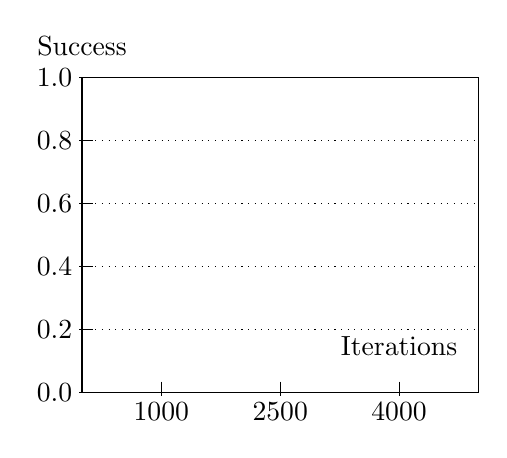
\begin{tikzpicture}[x=0.001cm,y=4cm]
    % Draw the axes and grid lines
    \draw[-] (0,0) -- (0,1) -- (5000,1) -- (5000,0) -- cycle; 
    \draw[-,thin, dotted, ystep=0.2, xstep=5000] (0,0) grid (5000,1);
    \foreach \x in {1000, 2500, 4000}  \draw [-,xshift=0](\x,4pt) -- (\x,-1pt);
    \foreach \y in {0.0,0.2,0.4,0.6,0.8,1.0}  \draw [-,yshift=0](4pt,\y) -- (-1pt,\y);
    \foreach \x/\xtext in {1000/1000, 2500/2500, 4000/4000} \node at (\x,0) [below] {$\xtext$};
    \foreach \y/\ytext in {0.0,0.2,0.4,0.6,0.8,1.0}  \node at (0,\y) [left] {$\ytext$};
    \node at (0,1.1) {Success};
    \node at (4000,0.15) {Iterations};
    \draw[-] plot[mark=x,mark size=4,mark options={color=black}] 
			file {data/hanoid5s1r8.CF.tikzdata};
    \draw[-] plot[mark=o,mark size=2,mark options={color=black}] 
			file {data/hanoid5s3r8.CF.tikzdata};
    \draw[-] plot[mark=+,mark size=2,mark options={color=black}] 
			file {data/hanoid5s5r8.CF.tikzdata};

\end{tikzpicture}

}
\caption{Agent performance under \CL\ and \CL+$\Omega$ schemes for solutions at recursion levels one (pluses), three (circles) and five (crosses). Each point represents results from $5$ experiment runs using an averaging window of $100$ samples.}
\end{center}
\end{figure*}

